\section{Summary of Fidler Leonardis }
\label{sec:fidler}
\todo[inline, author=Michael]{Draft. Please add some comments in todos.. need feedback}
This section aims to explain the work presented in \cite{fidler2009learning}. 
In their paper "Learning Hierarchical Compositional Representation of Object Structure" they proposed to use hierarchical compositionality (explained in section \ref{sec:hierarchical-comp}) for object recognition. 

\subsection{Hierarchical compositionality}
\label{sec:hierarchical-comp}
In essence, the term compositionality refers to complex parts made from combining other parts. \cite[p. 2]{fidler2007towards}
%\todo[inline, author=Michael]{Here is a tangent: 
The term is used within mathematics and languages as well, but here, only its use in extracting visual features is discussed. 
%} 

An example of combining multiple parts into a more complex part is shown in figure \ref{fig:compositionality1}. 
The letter "T" is formed or \textit{composed} from two simple line fragments. 
%Of course it would only make sense to compose a part from a group of parts if they are related. 
How to determine which parts to combine into a more complex part is discussed in section \ref{eqn:composition_of_parts}

\begin{figure}[h!] %compositionality1
\centering
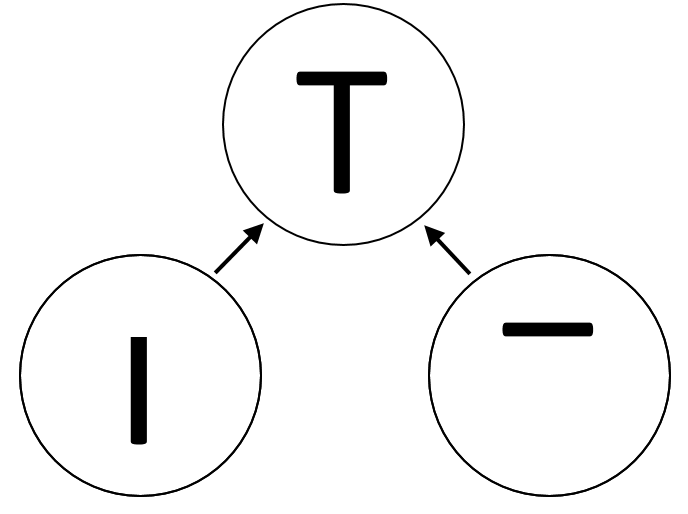
\includegraphics[width=0.3\textwidth]{graphics/compositionality1}
\caption{Combining two simple features into a more complex feature/composition.}
\label{fig:compositionality1}
\end{figure}

In (ref to paper) a hierarchy is built, combining features in a lower layer into more complex features in the layer above it. 
The motivation for using a hierarchy is discussed in section \ref{sec:deep_hierarchies}. 
Three different types of layers is used: 
\todo[inline, author=Michael]{I need a graphic here.. }

\paragraph*{The bottom layer} extracts simple features (edges) from the image. It uses a filter bank\footnote{A filter bank is simple an array of filters that splits the signal into different components. (ref: wikipedia filter bank)}
 consisting of 6 different Gabor filters of different orientation.\footnote{Gabor filters is a combination of a Sinus and a Gaussian distribution that is often used within computer vision for edge detection. (need ref)} 
The filter bank is shown in figure \ref{fig:filterbank}. 
This filter bank is applied directly to the image and the most prominent features is extracted. 
This is done by comparing the response of the filters with a threshold value, and thereby the sensitivity and number of extracted features can be controlled
This is repeated for different image scales, to be make the system robust towards the objects being of different sizes. 


The feature extraction/detection done at this layer is similar to the one of the PVC, namely the area V1. See section \ref{sec:pvc}. 


\begin{figure}[h!] %filterbank  %zoom = 400%
\centering
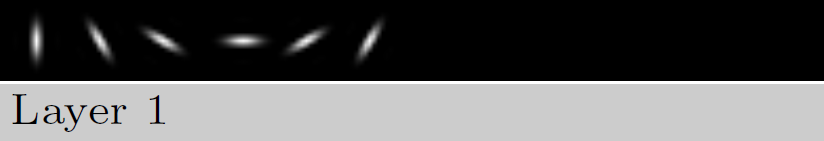
\includegraphics[width=0.4\textwidth]{graphics/layer1_features}
\caption{Filter bank used for feature extraction at layer 1.  
\cite[fig.~7]{fidler2009learning} }
\label{fig:filterbank}
\end{figure}

\paragraph*{Category independent layers} is located just above the bottom layer, and is learned without supervision. In the paper, Layer 2 and 3 is category independent layers.  The features is learned by combining parts from the layer below it (ie. Layer 2 is learned from Layer 1 features, Layer 3 from Layer 2 features etc.). This is described in section \ref{sec:composition-of-parts}. Examples of of layer 2 and 3 features is shown in figure \ref{fig:layer2+3}. 

The learning of these layers is unsupervised - this means that no input from humans is necessary when the layers are learned. Also, the layers are learned from a set of images containing a variety of objects. 


\begin{figure}[h!] %layer2 + 3  %zoom = 400%
	\centering
\begin{subfigure}[b]{0.3\textwidth}
	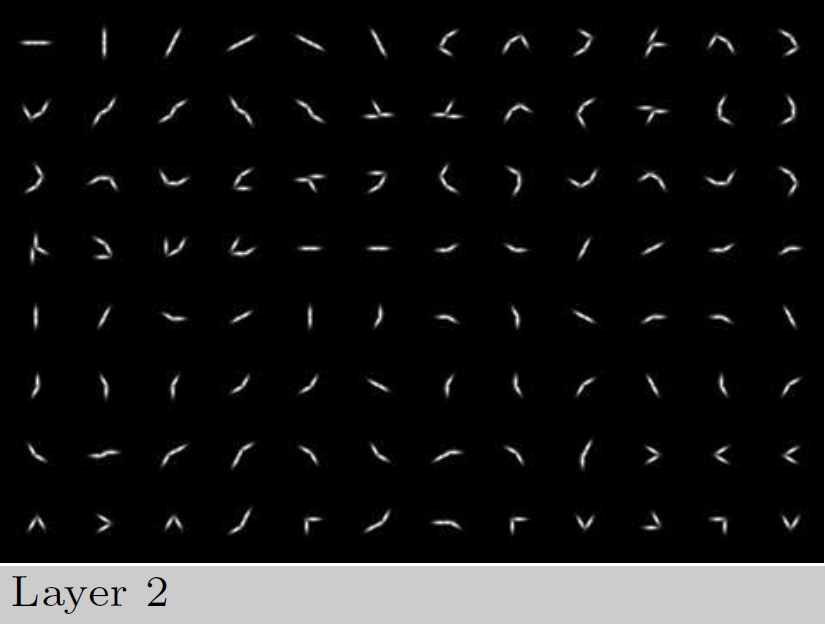
\includegraphics[height=4cm]{graphics/layer2_features}
	%\caption{blabla}
\end{subfigure}
\hspace{1cm}
\begin{subfigure}[b]{0.3\textwidth}
	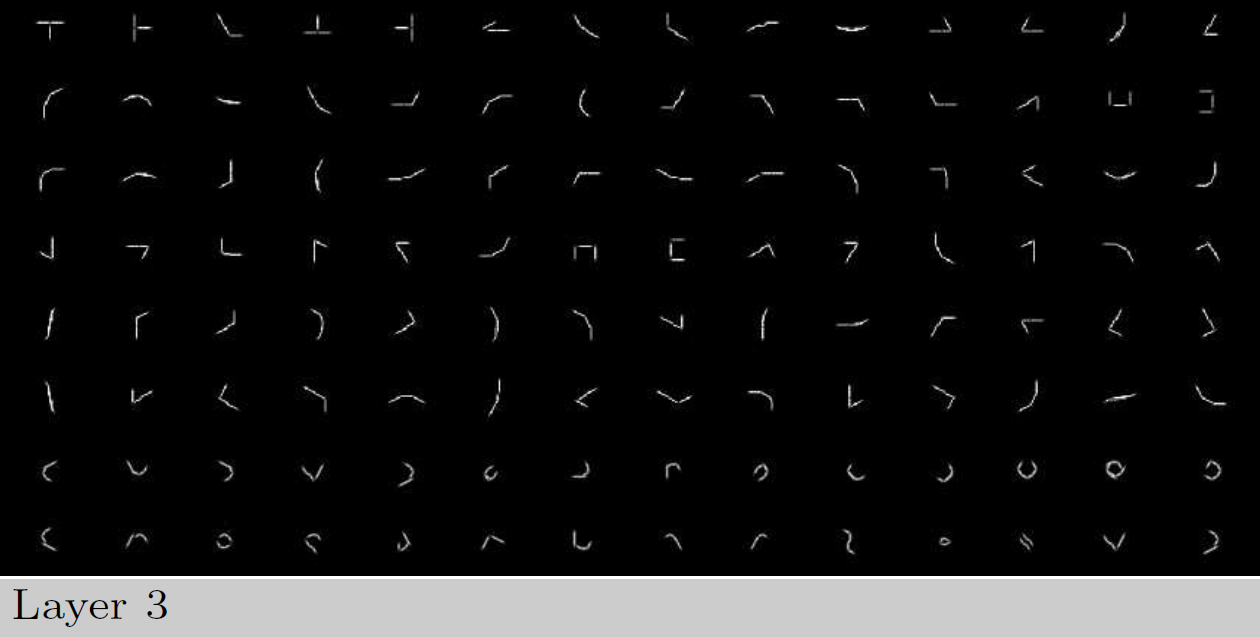
\includegraphics[height=4cm]{graphics/layer3_features}
	%\caption{blabla}
\end{subfigure}
\caption{Learned features in layer 2 and 3. 
\cite[fig.~7]{fidler2009learning} }
\label{fig:layer2+3}
\end{figure}

\paragraph*{Category specific layers} is the highest layers (4 and 5) of the hierarchy. These layers are learned from images of specific categories. The top-most layer combines the parts through the center of the object, to form the final object. 


\subsubsection{Composition of parts}
\label{sec:composition-of-parts}
Every part $\mathcal{P}_{\ell}^n$  in $\mathcal{L}_n$ (layer n) is composed of parts in $\mathcal{L}_{n-1}$. This means that all parts in $\mathcal{L}_5$  is compositions of parts in $\mathcal{L}_4$  and so forth
The composite part is made of a central part and its neighbours in the layer below. 
This list of sub-parts is shown in equation \ref{eqn:composition_of_parts}. 


\begin{equation}
\mathcal{P}_{\ell}^n = \left(\mathcal{P}_{central}^{n-1} , \left\{\left(\mathcal{P}_j^{n-1}, \mu_j, \Sigma_j \right) \right\}_j \right)
\label{eqn:composition_of_parts}
\end{equation}
where $\mu = (x_j, y_j)$ is the relative position of sub-part $\mathcal{P}_{j}^{n-1}$. 
$\Sigma_j$ is the max allowed variance of its position around $(x_j, y_j)$. An example of a composite part is shown in figure \ref{fig:compositionality2} below.

\begin{figure}[h!] %composing part in layer 3
\centering
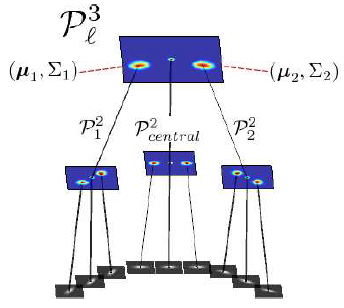
\includegraphics[scale=0.7]{graphics/compositionality2}
\caption{Example of a Layer 3 part, made from three Layer 2 parts. 
\cite[fig.~2]{fidler2009learning} }
\label{fig:compositionality2}
\end{figure}

To avoid (nearly) identical parts being learned multiple times in different compositions, the learned composition is grouped, based on similarity and co-occurrence. 
Compositions made up from the same sub-parts, but with different central parts, is grouped together. Parts often occurring together is also grouped. This grouping of parts lowers the number of parts in each layer, and makes the hierarchical representation more efficient. 

\subsubsection{Indexing and matching}
\label{sec:indexing-matching}
When the hierarchy is built, recognition of the items is done using a indexing and matching scheme. Recognizing objects in an image is done in the following steps: 

\begin{enumerate}
	\item Extract $\mathcal{L}_1$ features by applying the filter bank. A list of filters producing the maximum response and their position is saved as $\mathcal{L}_1$ parts. 
	\item Every found feature is checked against the parts found in the layer above. 
	Every part in $\mathcal{L}_{N}$  with part $\mathcal{P}_{\ell_k}^{n-1}$ as the central part is \textit{indexed}, yielding constant lookup time. 
	\item The parts $\mathcal{P}_{\ell}^{n}$ having part $\mathcal{P}_{\ell_k}^{n-1}$ as center is then \textit{matched}. In practice, this is done by checking if all sub-parts is presence in layer $\mathcal{L}_{N-1}$.
	\item Repeat step 2 + 3 for all remaining layers.  
\end{enumerate}

The process is also shown in figure \ref{fig:indexing-matching}. 
\begin{figure}[h!] %composing part in layer 3
\centering
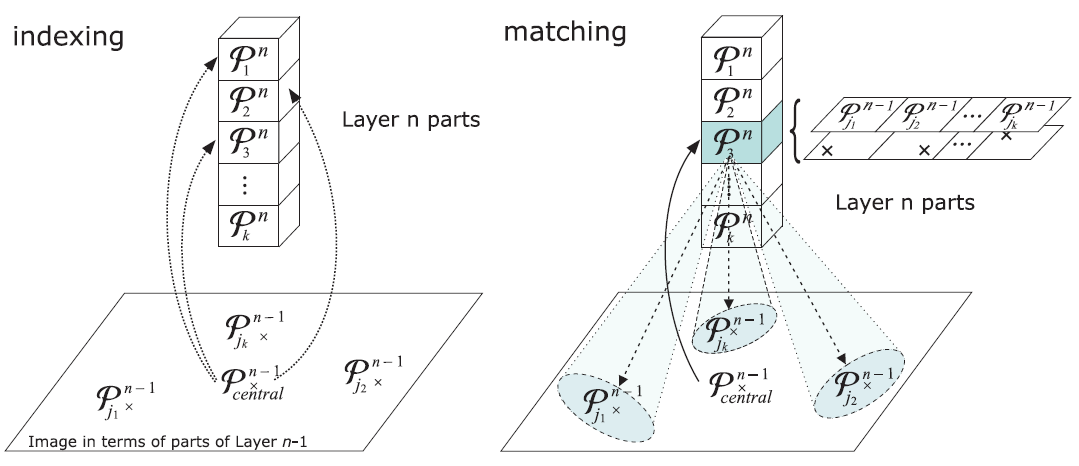
\includegraphics[width=0.8\textwidth]{graphics/indexing-matching}
\caption{The left side shows how a found feature $\mathcal{P}^{n-1}$ is against parts in $\mathcal{L}_{N-1}$ where it is the central parts. 
On the right side, the found part $\mathcal{P}_{3}^{n}$ is then matched against the neighbour features in $\mathcal{L}_{N-1}$. 
If all subparts is found in, the composite part is confirmed, and added to the list of found $\mathcal{L}_{N}$ features. \\
\cite[fig.~3]{fidler2009learning} }
\label{fig:indexing-matching}
\end{figure}

\subsection{Results of Fidler-Leonardis}
\label{sec:fidler-results}
To validate their approach, learning of the hierarchy was tested, using a set of 1500 images. 
The unsupervised part of the learned hierarchy consisted of 160 parts in Layer 2 and 553 parts in Layer 3. 
Some of the learned features is shown in figure \ref{fig:layer2+3}. 

The category specific layers was also tested. Multiple categories was learned, one of them being faces. 
The faces was learned by using 20 images containing faces. Parts in $\mathcal{L}_{4}$ was then used to learn $\mathcal{L}_{5}$ by  looking at the parts relative to the center of the face. 
The learned features for faces is shown in figure \ref{fig:layer4-5}.


\begin{figure}[h!] %faces layer 4 + 5
\centering
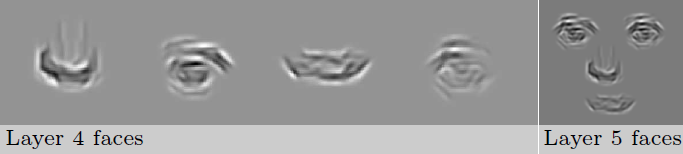
\includegraphics[scale=0.7]{graphics/layer4_5_faces}
\caption{Learned parts in $\mathcal{L}_{4}$ and $\mathcal{L}_{5}$ for recognizing faces. 
\cite[fig.~10]{fidler2009learning}}
\label{fig:layer4-5}
\end{figure}

